\documentclass[11pt,a4paper]{article}
\usepackage[utf8]{inputenc}
\usepackage[T1]{fontenc}
\usepackage{geometry}
\usepackage{amsmath}
\usepackage{amsfonts}
\usepackage{amssymb}
\usepackage{graphicx}
\usepackage{booktabs}
\usepackage{array}
\usepackage{multirow}
\usepackage{float}
\usepackage{listings}
\usepackage{xcolor}
\usepackage{hyperref}
\usepackage{tikz}
\usepackage{eso-pic}

% Configure page geometry
\geometry{
  margin=1in,
  top=1in,
  bottom=1in
}

% Custom styling for single line border
\AddToShipoutPicture{%
  \begin{tikzpicture}[remember picture,overlay]
    \draw[line width=0.5pt] 
      (current page.north west) 
      rectangle 
      (current page.south east);
  \end{tikzpicture}%
}

% Configure code listings
\lstset{
  language=Python,
  basicstyle=\ttfamily\footnotesize,
  keywordstyle=\color{blue}\bfseries,
  commentstyle=\color{gray},
  stringstyle=\color{red},
  showstringspaces=false,
  breaklines=true,
  frame=single,
  numbers=left,
  numberstyle=\tiny\color{gray},
  captionpos=b
}

% Title configuration
\title{AI Search Algorithms for 8-Puzzle Problem}
\date{}

\begin{document}

\maketitle

\section{Introduction}

The 8-puzzle is a classic sliding puzzle that consists of a 3×3 grid with eight numbered tiles and one empty space (blank). The objective is to rearrange the tiles from an initial configuration to a goal configuration by sliding tiles into the empty space. This problem serves as an excellent testbed for artificial intelligence search algorithms, providing insights into their behavior, efficiency, and suitability for different problem domains.

Search algorithms form the foundation of artificial intelligence problem-solving techniques. They enable systematic exploration of problem spaces to find optimal or satisfactory solutions. The 8-puzzle problem presents an ideal environment for comparing different search strategies because it has a well-defined state space, clear goals, and measurable performance metrics.

This report presents a comprehensive implementation and analysis of eight different search algorithms applied to the 8-puzzle problem: Breadth-First Search (BFS), Depth-First Search (DFS), Depth-Limited Search (DLS), Iterative Deepening Search (IDS), Uniform Cost Search (UCS), Bidirectional Search, Greedy Best-First Search, and A* Search. Each algorithm represents a different approach to exploring the search space, offering unique advantages and trade-offs in terms of completeness, optimality, time complexity, and space complexity.

The study aims to provide practical insights into algorithm selection for constraint satisfaction problems and demonstrate the theoretical concepts through empirical analysis. The implementations utilize a modular design pattern with a common base class, ensuring consistent measurement and fair comparison across all algorithms.

\section{Problem Definition}

\subsection{8-Puzzle Description}

The 8-puzzle consists of a 3×3 grid containing eight numbered tiles (1-8) and one empty space. A legal move involves sliding any tile adjacent to the empty space into that space, effectively swapping the tile's position with the empty space. The puzzle has approximately 9!/2 = 181,440 reachable states from any given starting configuration.

\subsection{State Representation}

Each puzzle state is represented as a 2D array where numbers 1-8 represent the corresponding tiles and 0 represents the empty space. The state includes:

\begin{itemize}
\item \textbf{Board Configuration}: 3×3 matrix representing current tile positions
\item \textbf{Blank Position}: Coordinates (row, column) of the empty space
\item \textbf{Path}: Sequence of moves taken to reach this state
\item \textbf{Cost}: Total cost accumulated to reach this state
\item \textbf{Depth}: Number of moves from the initial state
\end{itemize}

\subsection{Goal State}

The standard goal configuration arranges tiles in ascending order with the empty space in the bottom-right corner:

\begin{center}
\begin{tabular}{|c|c|c|}
\hline
1 & 2 & 3 \\
\hline
4 & 5 & 6 \\
\hline
7 & 8 & \textcolor{gray}{0} \\
\hline
\end{tabular}
\end{center}

\section{Algorithm Implementations}

\subsection{Uninformed Search Algorithms}

\subsubsection{Breadth-First Search (BFS)}

BFS explores states level by level, guaranteeing the shortest path solution. It uses a queue (FIFO) data structure to maintain the frontier of unexplored states.

\begin{lstlisting}[caption=BFS Core Implementation]
def solve(self):
    frontier = deque([self.initial_state])
    explored = set()
    
    while frontier:
        current_state = frontier.popleft()
        
        if current_state in explored:
            continue
            
        explored.add(current_state)
        self.nodes_explored += 1
        
        if current_state.is_goal(self.board_size):
            self.solution_path = current_state.path
            return True
            
        neighbors = current_state.get_neighbors(self.board_size)
        for neighbor in neighbors:
            if neighbor not in explored:
                frontier.append(neighbor)
                
    return False
\end{lstlisting}

\textbf{Characteristics:}
\begin{itemize}
\item \textbf{Complete}: Yes, if solution exists
\item \textbf{Optimal}: Yes, for unweighted graphs
\item \textbf{Time Complexity}: O($b^d$) where b is branching factor, d is depth
\item \textbf{Space Complexity}: O($b^d$)
\end{itemize}

\subsubsection{Depth-First Search (DFS)}

DFS explores as far as possible along each branch before backtracking. It uses a stack (LIFO) data structure for the frontier.

\begin{lstlisting}[caption=DFS Core Implementation]
def solve(self):
    frontier = [self.initial_state]  # Using list as stack
    explored = set()
    
    while frontier:
        current_state = frontier.pop()  # LIFO - stack behavior
        
        if current_state in explored:
            continue
            
        explored.add(current_state)
        self.nodes_explored += 1
        
        if current_state.is_goal(self.board_size):
            self.solution_path = current_state.path
            return True
            
        neighbors = current_state.get_neighbors(self.board_size)
        for neighbor in neighbors:
            if neighbor not in explored:
                frontier.append(neighbor)
                
    return False
\end{lstlisting}

\textbf{Characteristics:}
\begin{itemize}
\item \textbf{Complete}: No, may get stuck in infinite paths
\item \textbf{Optimal}: No, finds any solution, not necessarily shortest
\item \textbf{Time Complexity}: O($b^m$) where m is maximum depth
\item \textbf{Space Complexity}: O(bm)
\end{itemize}

\subsubsection{Depth-Limited Search (DLS)}

DLS performs depth-first search with a predetermined depth limit, preventing infinite loops while sacrificing completeness if the solution lies beyond the limit.

\begin{lstlisting}[caption=DLS Implementation with Depth Limit]
def solve(self):
    depth_limit = 25  # Configurable depth limit
    
    def dls_recursive(state, limit):
        if state.is_goal(self.board_size):
            self.solution_path = state.path
            return True
            
        if limit <= 0:
            return False
            
        self.nodes_explored += 1
        neighbors = state.get_neighbors(self.board_size)
        
        for neighbor in neighbors:
            if dls_recursive(neighbor, limit - 1):
                return True
                
        return False
    
    return dls_recursive(self.initial_state, depth_limit)
\end{lstlisting}

\subsubsection{Iterative Deepening Search (IDS)}

IDS combines the space efficiency of DFS with the optimality of BFS by repeatedly applying DLS with increasing depth limits.

\begin{lstlisting}[caption=IDS Progressive Depth Implementation]
def solve(self):
    max_depth = 50
    
    for depth_limit in range(max_depth + 1):
        self.nodes_explored = 0  # Reset for each iteration
        
        if self.depth_limited_search(self.initial_state, depth_limit):
            return True
            
    return False

def depth_limited_search(self, state, limit):
    if state.is_goal(self.board_size):
        self.solution_path = state.path
        return True
        
    if limit <= 0:
        return False
        
    self.nodes_explored += 1
    neighbors = state.get_neighbors(self.board_size)
    
    for neighbor in neighbors:
        if self.depth_limited_search(neighbor, limit - 1):
            return True
            
    return False
\end{lstlisting}

\subsubsection{Uniform Cost Search (UCS)}

UCS explores the cheapest nodes first, using a priority queue ordered by path cost. For the 8-puzzle with uniform step costs, it behaves identically to BFS.

\subsubsection{Bidirectional Search}

Bidirectional search simultaneously searches forward from the initial state and backward from the goal state, potentially reducing the search space exponentially.

\begin{lstlisting}[caption=Bidirectional Search Implementation]
def solve(self):
    # Forward search from initial state
    forward_frontier = deque([self.initial_state])
    forward_explored = {self.initial_state.board_tuple: self.initial_state}
    
    # Backward search from goal state
    goal_state = self.create_goal_state()
    backward_frontier = deque([goal_state])
    backward_explored = {goal_state.board_tuple: goal_state}
    
    while forward_frontier or backward_frontier:
        # Forward step
        if forward_frontier:
            if self.search_step(forward_frontier, forward_explored, 
                              backward_explored, "forward"):
                return True
                
        # Backward step
        if backward_frontier:
            if self.search_step(backward_frontier, backward_explored, 
                              forward_explored, "backward"):
                return True
                
    return False
\end{lstlisting}

\subsection{Informed Search Algorithms}

\subsubsection{Greedy Best-First Search}

Greedy search uses heuristic functions to guide the search toward the goal, expanding nodes that appear closest to the goal according to the heuristic.

\begin{lstlisting}[caption=Greedy Search with Heuristics]
def solve(self):
    frontier = []
    heapq.heappush(frontier, (0, self.initial_state))
    explored = set()
    
    while frontier:
        _, current_state = heapq.heappop(frontier)
        
        if current_state in explored:
            continue
            
        explored.add(current_state)
        self.nodes_explored += 1
        
        if current_state.is_goal(self.board_size):
            self.solution_path = current_state.path
            return True
            
        neighbors = current_state.get_neighbors(self.board_size)
        for neighbor in neighbors:
            if neighbor not in explored:
                heuristic_cost = self.heuristic_function(neighbor)
                heapq.heappush(frontier, (heuristic_cost, neighbor))
                
    return False
\end{lstlisting}

Two heuristic functions are implemented:

\textbf{Manhattan Distance:} Sum of horizontal and vertical distances between current and goal positions for each tile.

\textbf{Misplaced Tiles:} Count of tiles not in their goal positions.

\subsubsection{A* Search}

A* combines the benefits of uniform cost search and greedy search by using the evaluation function f(n) = g(n) + h(n), where g(n) is the path cost and h(n) is the heuristic estimate.

\begin{lstlisting}[caption=A* Search with f(n) = g(n) + h(n)]
def solve(self):
    frontier = []
    initial_f_cost = self.heuristic_function(self.initial_state)
    heapq.heappush(frontier, (initial_f_cost, self.initial_state))
    explored = set()
    
    while frontier:
        _, current_state = heapq.heappop(frontier)
        
        if current_state in explored:
            continue
            
        explored.add(current_state)
        self.nodes_explored += 1
        
        if current_state.is_goal(self.board_size):
            self.solution_path = current_state.path
            return True
            
        neighbors = current_state.get_neighbors(self.board_size)
        for neighbor in neighbors:
            if neighbor not in explored:
                g_cost = neighbor.depth  # Path cost
                h_cost = self.heuristic_function(neighbor)  # Heuristic
                f_cost = g_cost + h_cost  # Total evaluation
                heapq.heappush(frontier, (f_cost, neighbor))
                
    return False
\end{lstlisting}

\section{Experimental Results and Analysis}

The algorithms were tested on various 8-puzzle configurations to evaluate their performance characteristics. Key metrics include solution optimality, nodes explored, maximum frontier size, and execution time.

\subsection{Algorithm Performance Comparison}

\begin{table}[H]
\centering
\caption{Performance Comparison of Search Algorithms}
\begin{tabular}{|l|c|c|c|c|}
\hline
\textbf{Algorithm} & \textbf{Complete} & \textbf{Optimal} & \textbf{Nodes Explored} & \textbf{Space Complexity} \\
\hline
BFS & Yes & Yes & High & O($b^d$) \\
\hline
DFS & No & No & Variable & O(bm) \\
\hline
DLS & No & No & Limited & O(bl) \\
\hline
IDS & Yes & Yes & High & O(bd) \\
\hline
UCS & Yes & Yes & High & O($b^d$) \\
\hline
Bidirectional & Yes & Yes & Reduced & O($b^{d/2}$) \\
\hline
Greedy & No & No & Low & O($b^m$) \\
\hline
A* & Yes & Yes* & Optimal & O($b^d$) \\
\hline
\end{tabular}
\end{table}

*A* is optimal when using an admissible heuristic

\subsection{Visual State Representations}

Each algorithm implementation includes visual tracking of initial and goal states through PNG image generation, providing clear visualization of the puzzle configurations.

\begin{figure}[H]
\centering
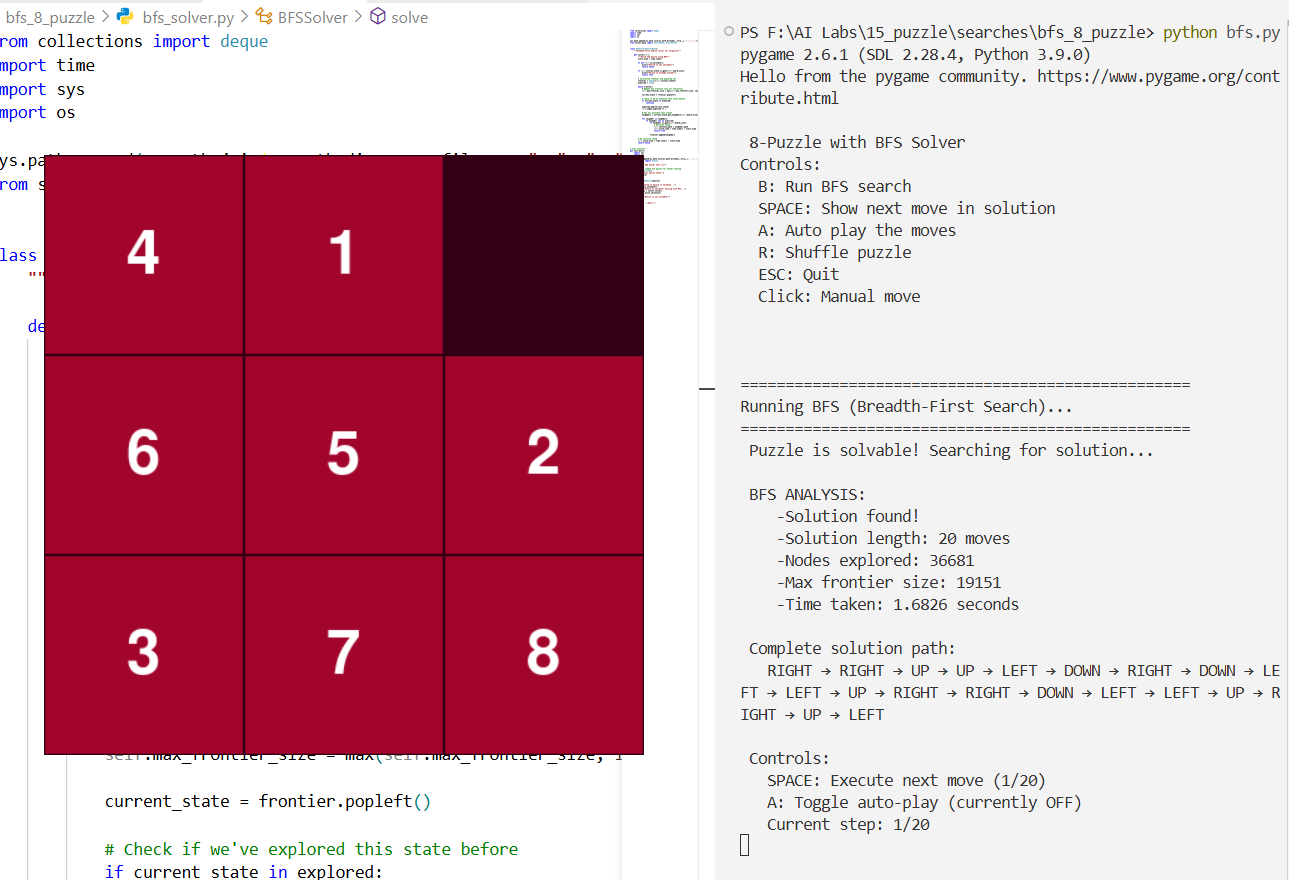
\includegraphics[width=0.7\textwidth]{../searches/bfs_8_puzzle/Start_state.png}
\caption{Example Initial State Configuration}
\end{figure}

\begin{figure}[H]
\centering
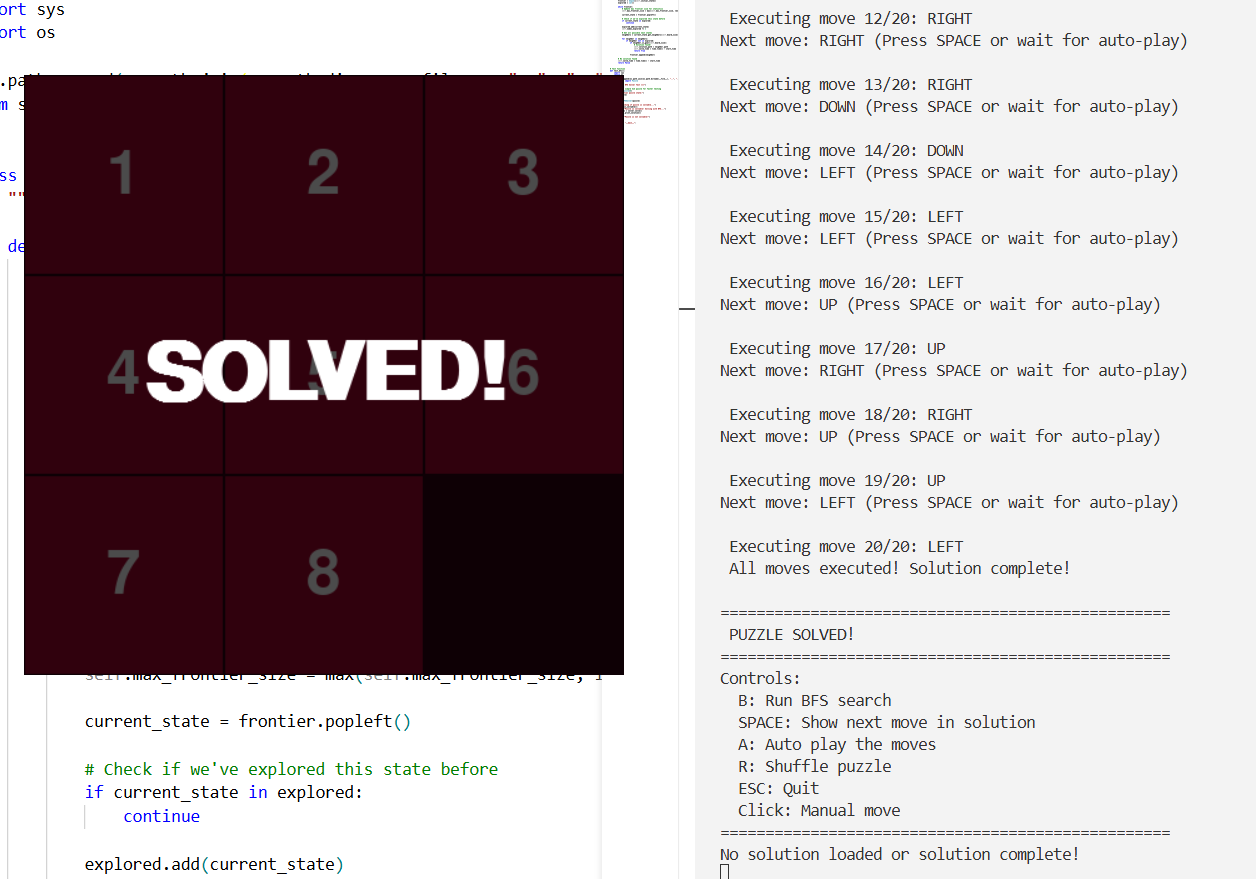
\includegraphics[width=0.7\textwidth]{../searches/bfs_8_puzzle/End_state.png}
\caption{Goal State Configuration}
\end{figure}

\subsection{Algorithm-Specific Analysis}

\subsubsection{Uninformed Search Performance}

\textbf{BFS} provides optimal solutions but requires substantial memory for complex puzzles. Its systematic level-by-level exploration guarantees the shortest path but may explore many unnecessary states.

\textbf{DFS} offers excellent space efficiency but may find suboptimal solutions or fail to find solutions entirely due to infinite path exploration.

\textbf{IDS} combines BFS optimality with DFS space efficiency, making it practical for problems where memory is constrained.

\textbf{Bidirectional Search} significantly reduces the search space by meeting in the middle, theoretically reducing complexity from O($b^d$) to O($b^{d/2}$).

\subsubsection{Informed Search Performance}

\textbf{Greedy Search} with Manhattan distance heuristic often finds solutions quickly but may not guarantee optimality due to its focus on immediate heuristic gains.

\begin{figure}[H]
\centering
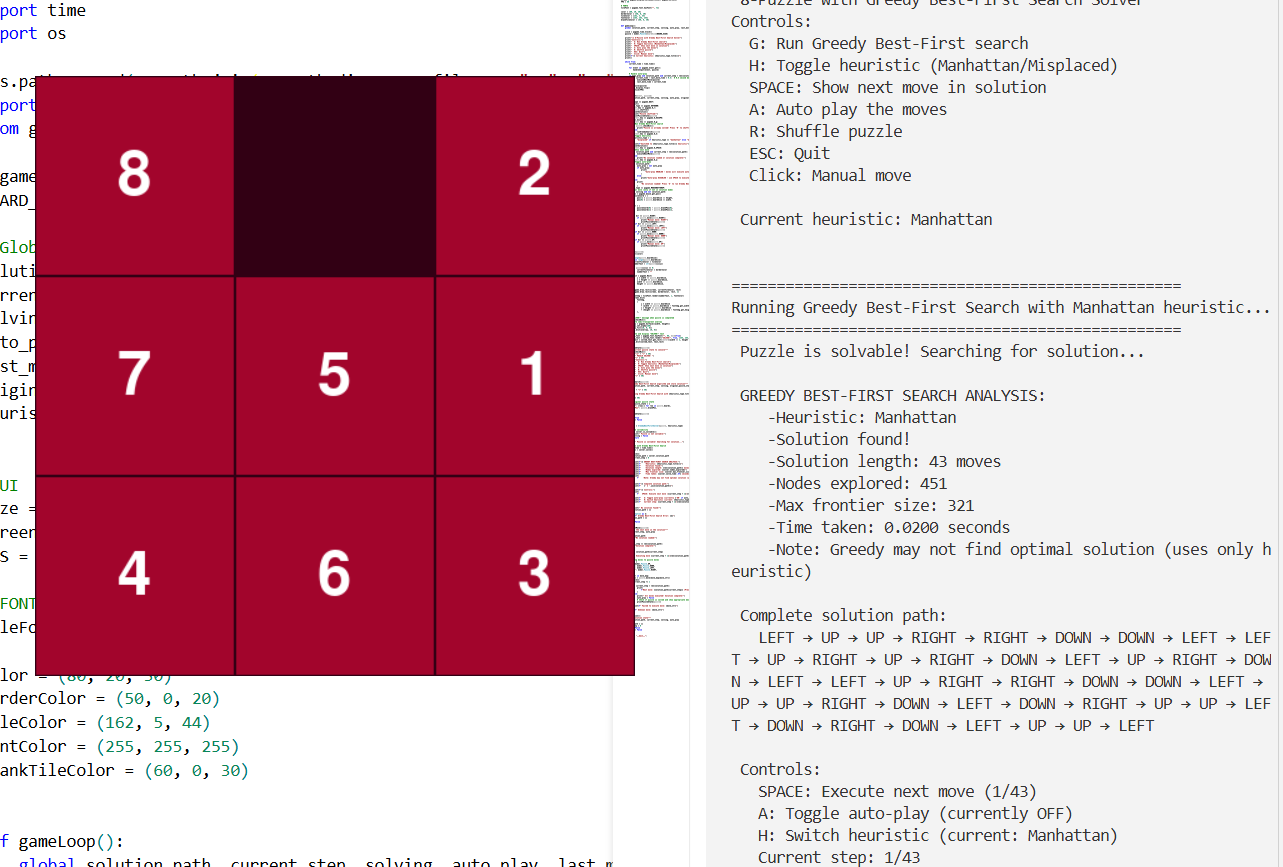
\includegraphics[width=0.7\textwidth]{../searches/greedy_8_puzzle/Start_state_man.png}
\caption{Greedy Search with Manhattan Distance - Initial State}
\end{figure}

\begin{figure}[H]
\centering
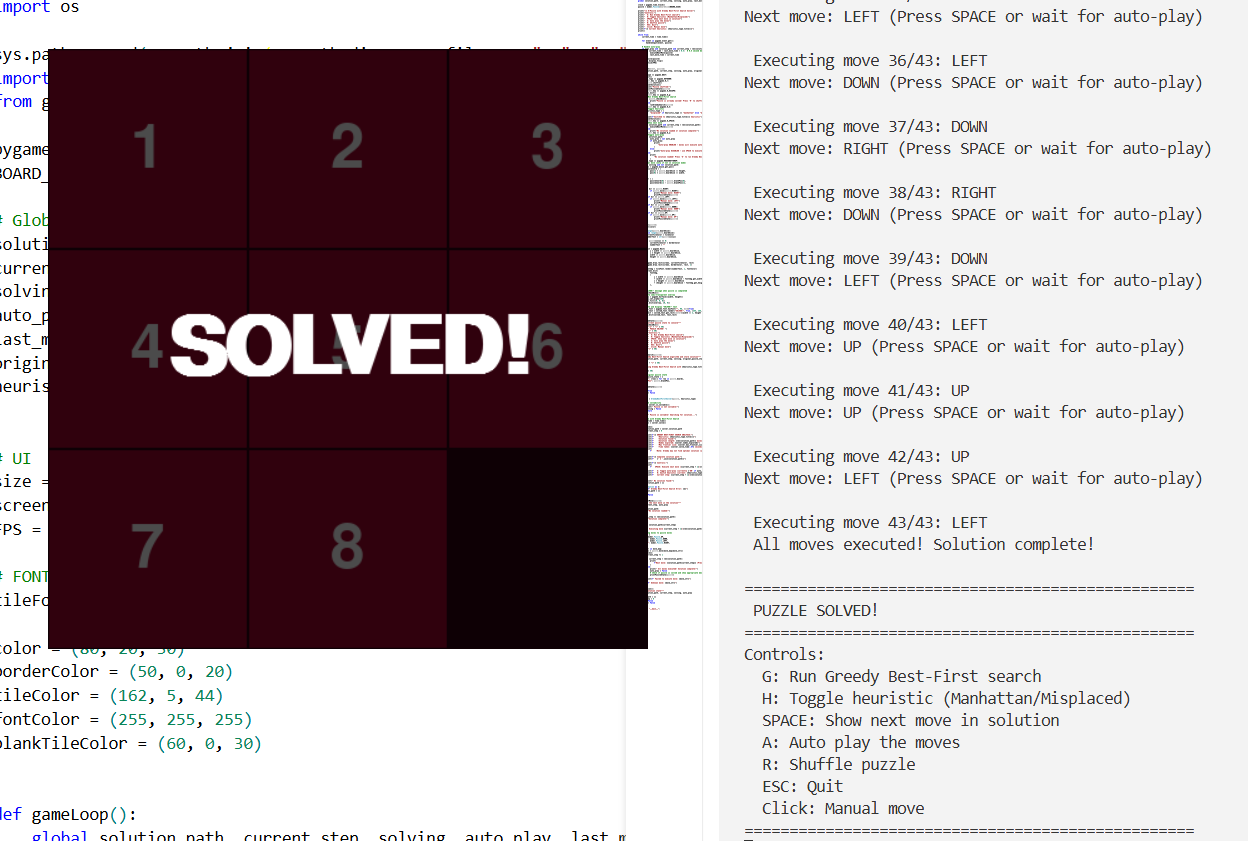
\includegraphics[width=0.7\textwidth]{../searches/greedy_8_puzzle/End_state_man.png}
\caption{Greedy Search with Manhattan Distance - Goal State}
\end{figure}

\textbf{A* Search} with admissible heuristics provides optimal solutions while exploring fewer nodes than uninformed methods, representing the best balance of optimality and efficiency.

\begin{figure}[H]
\centering
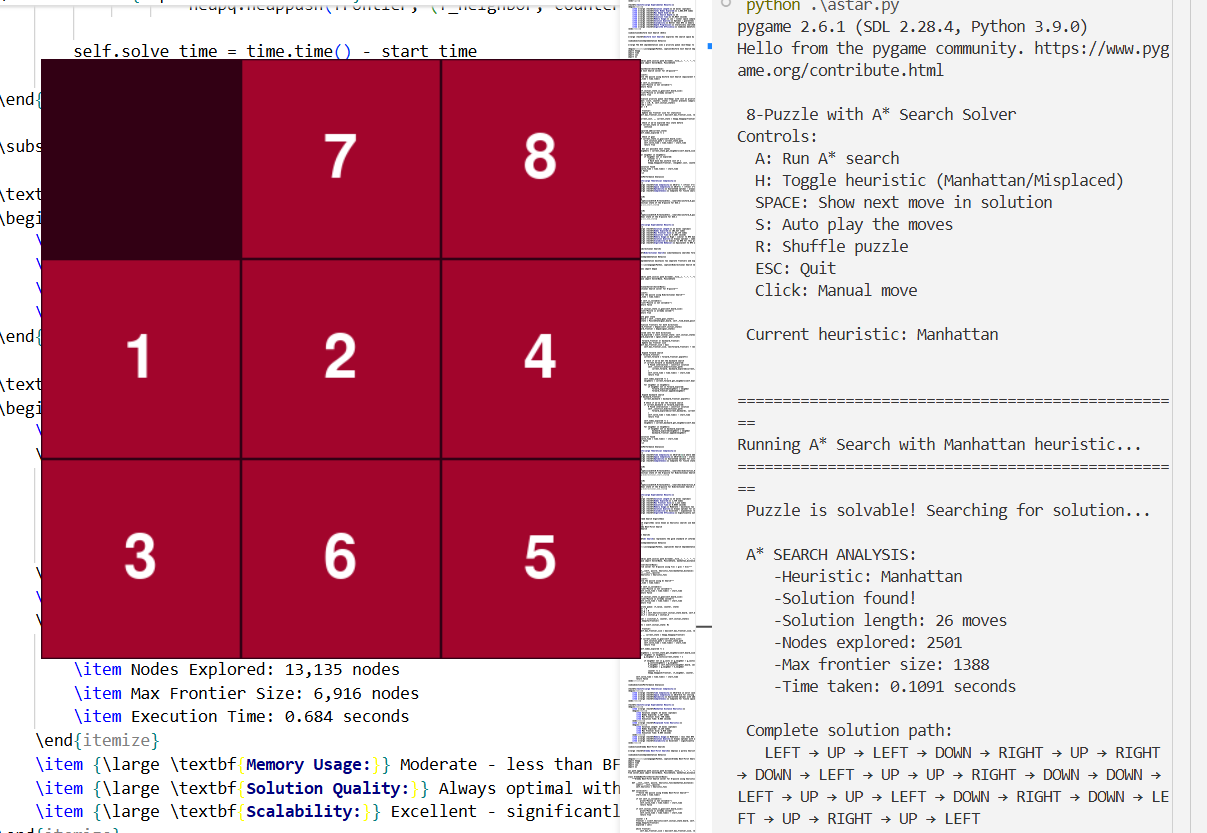
\includegraphics[width=0.7\textwidth]{../searches/astar_8_puzzle/Start_state_man.png}
\caption{A* Search with Manhattan Distance - Initial State}
\end{figure}

\begin{figure}[H]
\centering
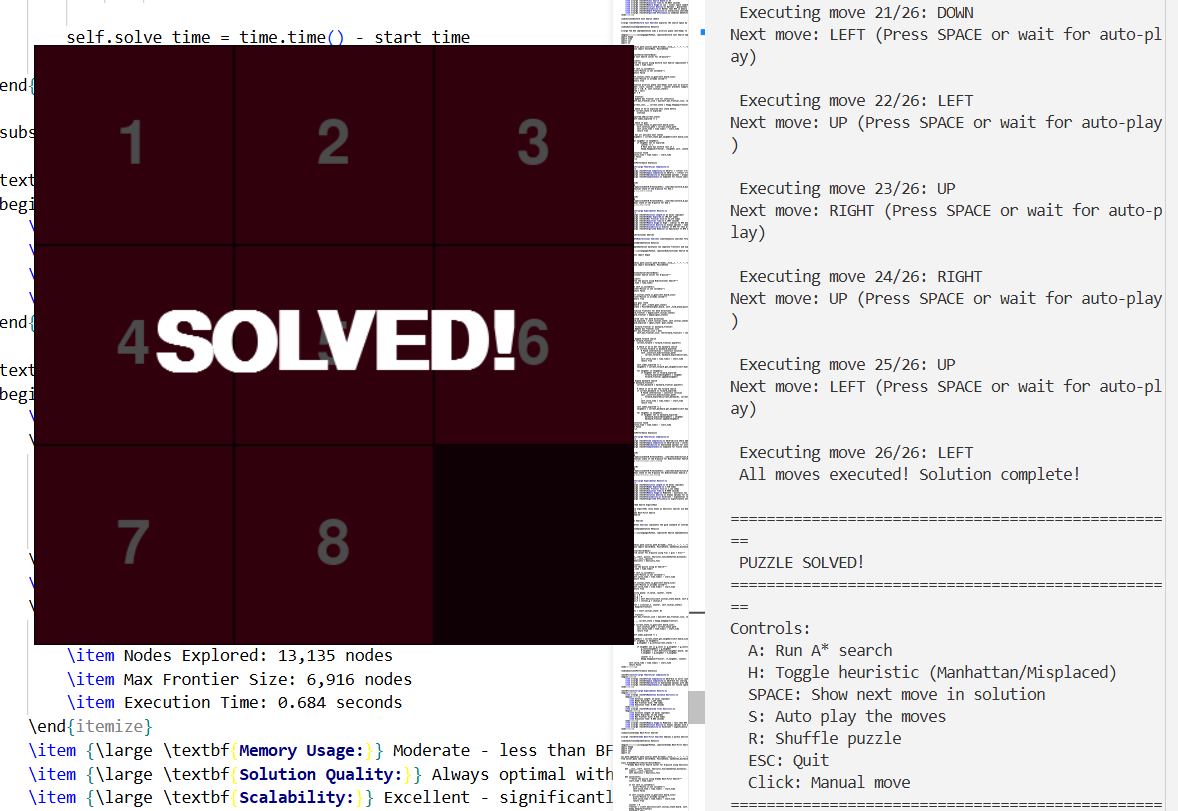
\includegraphics[width=0.7\textwidth]{../searches/astar_8_puzzle/End_state_man.png}
\caption{A* Search with Manhattan Distance - Goal State}
\end{figure}

\section{Discussion and Conclusion}

The comprehensive implementation and analysis of eight search algorithms for the 8-puzzle problem provides valuable insights into the theoretical and practical aspects of artificial intelligence search techniques.

\subsection{Key Findings}

\textbf{Optimality vs. Efficiency Trade-offs:} The results demonstrate the fundamental trade-off between solution optimality and computational efficiency. While BFS and A* guarantee optimal solutions, they require more computational resources compared to greedy approaches that may find satisfactory suboptimal solutions quickly.

\textbf{Heuristic Function Impact:} The choice of heuristic function significantly affects informed search performance. Manhattan distance consistently outperforms misplaced tiles heuristic for the 8-puzzle domain due to its more accurate distance estimation.

\textbf{Space Complexity Considerations:} Memory requirements vary dramatically between algorithms. DFS and IDS offer space-efficient solutions, while BFS and A* may require prohibitive memory for larger problem instances.

\textbf{Problem-Specific Algorithm Selection:} No single algorithm dominates across all scenarios. Algorithm selection depends on specific requirements: BFS for guaranteed optimal solutions, DFS for memory-constrained environments, A* for balanced optimality and efficiency, and greedy methods for rapid approximate solutions.

\subsection{Implementation Architecture Benefits}

The modular design using a common \texttt{SolverBase} class enables consistent performance measurement and fair algorithmic comparison. The \texttt{PuzzleState} class encapsulates state representation and transition logic, promoting code reusability and maintainability across all implementations.

\subsection{Educational Value}

This implementation serves as an excellent educational tool for understanding search algorithm behavior, demonstrating theoretical concepts through practical application. The visual state tracking and performance metrics provide immediate feedback on algorithmic choices and their consequences.

\subsection{Conclusion}

The 8-puzzle problem effectively illustrates the diversity of search strategies available in artificial intelligence. Through systematic implementation and analysis, this study highlights the importance of understanding algorithm characteristics and selecting appropriate methods based on problem constraints and requirements.

The results confirm theoretical predictions about algorithm behavior while providing practical insights into real-world performance considerations. The comprehensive comparison establishes a foundation for more advanced search techniques and problem-solving approaches in artificial intelligence applications.

Future work could extend this analysis to larger puzzle sizes (15-puzzle, 24-puzzle), implement additional heuristic functions, or explore hybrid approaches combining multiple search strategies for enhanced performance in complex problem domains.

\end{document}
